\newcommand{\msg}[2]{%
  \ifthenelse
    {\isempty{#1}}
    {\ensuremath{(#2)}}
    {\ifthenelse
      {\isempty{#2}}
      {\ensuremath{(\mathsf{#1})}}
      {\ensuremath{(\mathsf{#1}, #2)}}
    }
}

%----- Comments ----------------------------------------------------------------
\RequirePackage{totcount}
\RequirePackage{color}
\RequirePackage[disable]{todonotes}

\newtotcounter{notecount}
\newcommand{\notewarning}{%
\ifnum\totvalue{notecount}>0%
 \vspace{1ex}
\begin{center}
 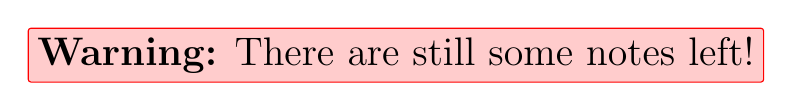
\begin{tikzpicture}[baseline=(A.south)]
    \node (A) [] at (0,0){};
    \node [rounded corners=1pt,rectangle, draw=red, fill=red!20,text=black](B) at (0.1ex,0ex){
        \Large \raggedright {\bf Warning:} There are still some notes left!
    };
 \end{tikzpicture}
\end{center}
 \vspace{1ex}
\fi
}
\makeatletter
\def\myaddcontentsline#1#2#3{%
  \addtocontents{#1}{\protect\contentsline{#2}{#3}{Section \thesubsection\ at p. \thepage}{}}}
\makeatother
\definecolor{lightgreen}{rgb}{0.86, 0.93, 0.78}
\definecolor{bordergreen}{rgb}{0.55, 0.76, 0.74}
\definecolor{lightblue}{rgb}{0.70, 0.90, 0.99}
\definecolor{borderblue}{rgb}{0.01, 0.66, 0.96}
\definecolor{lightamber}{rgb}{1, 0.93, 0.70}
\definecolor{borderamber}{rgb}{1, 0.76, 0.03}
\definecolor{lightcolor4}{rgb}{ 0.93, 0.70, 1}
\definecolor{bordercolor4}{rgb}{0.76, 0.03, 1}

% \newcommand{\note}[1]{\stepcounter{notecount}\todo[inline,bordercolor=bordergreen,linecolor=bordergreen,color=lightgreen]{ #1}{}}
% \newcommand{\snote}[1]{\stepcounter{notecount}\todo[bordercolor=bordergreen,linecolor=bordergreen,color=lightgreen,fancyline]{ #1}{}}

\newcommand{\mnote}[1]{
  \stepcounter{notecount}
  \todo[
        inline,
        caption={minipage-note},
        bordercolor=bordergreen,
        linecolor=bordergreen,
        color=lightgreen,
        fancyline
      ]
      {
        \begin{minipage}{0.9\textwidth}
           #1
        \end{minipage}
      }
      {}
}

\def\showauthnotes{1}
\ifthenelse{\showauthnotes=1}
{
  \newcommand{\authnote}[2]{\mnote{\textbf{#1:} #2}}
%\newcommand{\authnote}[2]{{ \footnotesize \bf{[#1: #2]~}}}
%\newcommand{\authnote}[2]{{ \tt {[#1: #2]~}}}
}

\newcommand{\dionyziz}[1]{\authnote{Dionysis}{#1}}
\newcommand{\dimitris}[1]{\authnote{Dimitris}{#1}}
\newcommand{\christos}[1]{\authnote{Christos}{#1}}
\newcommand{\aggelos}[1]{\authnote{Aggelos}{#1}}

\newcommand{\TODO}[1]{
  \if\relax\detokenize{#1}\relax
    \textcolor{red}{TODO}
  \else
    \textcolor{red}{ {#1}}
  \fi
}

%---------------------------------------------------------------------

\newcommand{\footTODO}[1]{\footnote{\TODO{#1}}}

\newcommand{\ignore}[1]{}



% the \Bot symbol from https://tex.stackexchange.com/questions/297971/bot-like-symbol-with-two-horizontal-lines
\makeatletter
\DeclareRobustCommand{\Bot}{%
  \mathord{\vphantom{\bot}\mathpalette\mich@Bot\relax}%
}
\newcommand{\mich@Bot}[2]{%
  \ooalign{%
    $\m@th#1\bot$\cr
    \clipbox*{0pt 0pt {\width} {.5\height}}{\raisebox{.2\height}{$\m@th#1\bot$}}\cr
  }%
}
\makeatother

\newcommand{\ec}{\textsc{ec}}
\newcommand{\bgr}{\textsc{bgr}}
\newcommand{\thr}{\textsc{thr}}
\newcommand{\br}{\textsc{br}}
\newcommand{\tp}{\textsc{tp}}
\newcommand{\ecr}{\textsc{ecr}}
\newcommand{\hr}{\textsc{hr}}
\newcommand{\ir}{\textsc{ir}}
\newcommand{\ic}{\textsc{ic}}
\newcommand{\eg}{e.g. }
\newcommand{\ie}{i.e., }

\newcommand{\placefigure}[4]{
  \iflncs
    \begin{figure}[H]
        \caption{#3}
        \centering
        \includegraphics[width=#4 \columnwidth,keepaspectratio]{figures/#1}
        \label{#2}
    \end{figure}
  \else
    \begin{figure}
        \caption{#3}
        \centering
        \includegraphics[width=#4 \columnwidth,keepaspectratio]{figures/#1}
        \label{#2}
    \end{figure}
  \fi
}

\newcommand{\conc}{\mathbin{\|}}

\newcommand{\hash}{\mathsf{H}}
\newcommand{\xor}{\oplus}
\newcommand{\true}{\mathsf{true}}
\newcommand{\false}{\mathsf{false}}

\newcommand{\kv}[2] { #1{:}\,#2 }

\newcommand{\Gen}{\mathsf{Gen}}
\newcommand{\Sig}{\mathsf{Sig}}
\newcommand{\Ver}{\mathsf{Ver}}

\newcommand{\GenAddr}{\mathsf{GenAddr}}
\newcommand{\SpendVerify}{\mathsf{SpendVerify}}
\newcommand{\GenBurnAddr}{\mathsf{Gen}\-\mathsf{Burn}\-\mathsf{Addr}}
\newcommand{\BurnVerify}{\mathsf{BurnVerify}}
\newcommand{\burnAddr}{\mathsf{burnAddr}}

\newcommand{\cind}{\approx_c}
\newcommand{\query}{\textsc{qry}}

\newcommand{\uniform}{\mathcal{U}}
\newcommand{\uniformk}{\uniform(\{0,1\}^\kappa)}
\newcommand{\extqry}{\textsc{exqry}}
\newcommand{\negl}{\textsf{negl}(\kappa)}

\newcommand{\spendattack}{\textsc{spend}\-\text{-}\-\textsc{attack}}
\newcommand{\bindattack}{\textsc{bind}\-\text{-}\-\textsc{attack}}
\newcommand{\collisionattack}{\textsf{collision}}
\newcommand{\predict}{\textsc{predict}}
\newcommand{\distattack}{\textsc{dist}\-\text{-}\-\textsc{game}}

\newcommand{\VerMT}{\mathsf{Ver}\mathcal{MT}}
\newcommand{\VerTxIncl}{\mathsf{VerTxIncl}}
\newcommand{\TxHasTransfer}{\mathsf{TxHasTransfer}}

\newcommand{\tx}{\textsf{tx}}

\newcommand{\checksum}{\textsf{checksum}}
\newcommand{\addr}{\textsf{addr}}

\newcommand{\SHA}{\texttt{SHA256}}
\newcommand{\RIPEMD}{\texttt{RIPEMD160}}
\newcommand{\BTCHASH}{\texttt{HASH160}}
\newcommand{\baseencode}{\texttt{base58}}

\newcommand{\Mod}[1]{\ (\mathrm{mod}\ #1)}
